\documentclass[final]{beamer}

\usepackage[scale=1.24]{beamerposter} % Use the beamerposter package for laying out the poster
\usepackage{wrapfig}
\usepackage{subcaption}
\usetheme{confposter} % Use the confposter theme supplied with this template

\setbeamercolor{block title}{fg=ucdblue,bg=white} % Colors of the block titles
\setbeamercolor{block body}{fg=black,bg=white} % Colors of the body of blocks
\setbeamercolor{block alerted title}{fg=ucdgold,bg=ucdblue} % Colors of the highlighted block titles
\setbeamercolor{block alerted body}{fg=black,bg=ucdblue!10} % Colors of the body of highlighted blocks
% Many more colors are available for use in beamerthemeconfposter.sty
\setbeamertemplate{caption}[numbered] 
%-----------------------------------------------------------
% Define the column widths and overall poster size
% To set effective sepwid, onecolwid and twocolwid values, first choose how many columns you want and how much separation you want between columns
% In this template, the separation width chosen is 0.024 of the paper width and a 4-column layout
% onecolwid should therefore be (1-(# of columns+1)*sepwid)/# of columns e.g. (1-(4+1)*0.024)/4 = 0.22
% Set twocolwid to be (2*onecolwid)+sepwid = 0.464
% Set threecolwid to be (3*onecolwid)+2*sepwid = 0.708

\newlength{\sepwid}
\newlength{\onecolwid}
\newlength{\twocolwid}
\newlength{\threecolwid}
\setlength{\paperwidth}{48in} % A0 width: 46.8in
\setlength{\paperheight}{36in} % A0 height: 33.1in
\setlength{\sepwid}{0.012\paperwidth} % Separation width (white space) between columns
\setlength{\onecolwid}{0.22\paperwidth} % Width of one column
\setlength{\twocolwid}{0.464\paperwidth} % Width of two columns
\setlength{\threecolwid}{0.708\paperwidth} % Width of three columns
\setlength{\topmargin}{-0.5in} % Reduce the top margin size
%-----------------------------------------------------------

\usepackage{graphicx}  % Required for including images

\usepackage{booktabs} % Top and bottom rules for tables

\usepackage{subcaption}

\usepackage{natbib}

\usepackage[export]{adjustbox}
 	
\setbeamerfont{caption}{size=\small}
%----------------------------------------------------------------------------------------
%	TITLE SECTION 
%----------------------------------------------------------------------------------------

\title{Arctic Mixed-Phase Cloud Dissipation and its Relationship to Low CCN Concentrations} % Poster title

\author{\textbf{Lucas Sterzinger}, Adele L. Igel} % Author(s)

\institute{Atmospheric Science Graduate Group \\ Department of Land, Air, and Water Resources - University of California, Davis} % Institution(s)

%----------------------------------------------------------------------------------------

\begin{document}
%\setbeamercolor{background canvas}{bg=ucdgold!20}
\addtobeamertemplate{block end}{}{\vspace*{2ex}} % White space under blocks
\addtobeamertemplate{block alerted end}{}{\vspace*{2ex}} % White space under highlighted (alert) blocks

\setlength{\belowcaptionskip}{2ex} % White space under figures
\setlength\belowdisplayshortskip{2ex} % White space under equations

\begin{frame}[t] % The whole poster is enclosed in one beamer frame

\begin{columns}[t] % The whole poster consists of three major columns, the second of which is split into two columns twice - the [t] option aligns each column's content to the top

\begin{column}{\sepwid}\end{column} % Empty spacer column

\begin{column}{\onecolwid} % The first column

%----------------------------------------------------------------------------------------
%	OBJECTIVES
%----------------------------------------------------------------------------------------
    \begin{alertblock}{Overview}
	\textit{Can a lack of environmental CCN/aerosol be a primary factor for Arctic cloud dissipation?}
	        \begin{itemize}
            \item Persistent mixed-phase boundary layer clouds are important regulators for Arctic (and global) climate.
            \item Accurately modeling Arctic clouds are important to properly simulate the global climate system.
            \item Unlike in lower latitudes, Arctic aerosol concentrations have been hypothesized to be low enough to inhibit cloud formation
			\begin{itemize}
				\item Mauritsen et al. (2011) coined the term "tenuous clouds" in which cloud structure was limited by aerosol concentration
			\end{itemize}
        \end{itemize}
	\end{alertblock}
	
	\begin{block}{Cases and Simulation Setup}
		Two potential cases have been identified where cloud dissipation occurred coincidentally with a surface aerosol concentration decrease:
		\begin{itemize}
			\item Oliktok Point - May 12th, 2017
			\begin{itemize}
				\item Northern slope of Alaska - ocean/land boundary
			\end{itemize}
			\item ASCOS - August 31st, 2008
			\begin{itemize}
				\item Arctic ocean ice floe
			\end{itemize}
		\end{itemize}
		
		The plots below show radar reflectivity (a) and aerosol concentration (b).
		\begin{figure}
			\includegraphics[width=0.9\linewidth]{images/oli_timeseries.png}
			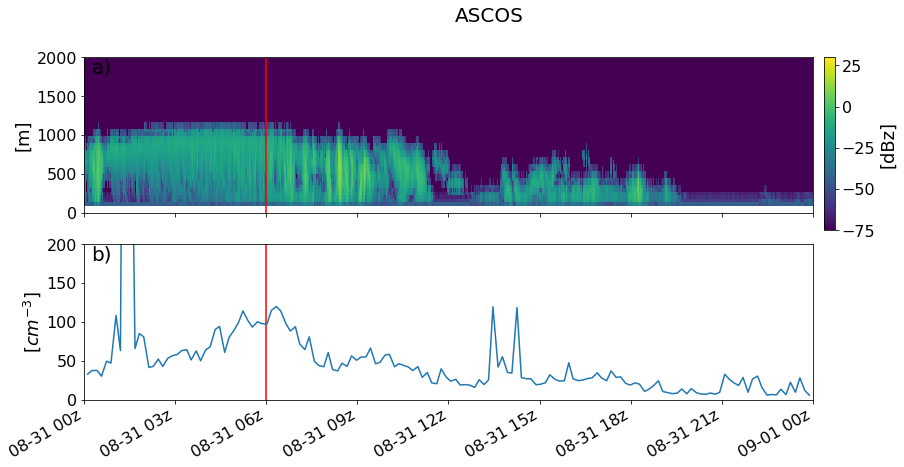
\includegraphics[width=0.9\linewidth]{images/ascos_timeseries.png}

		\end{figure}
	\end{block}
\end{column} % End of the first column

\begin{column}{\sepwid}\end{column} % Empty spacer column

\begin{column}{\twocolwid}
\begin{block}{Simulation Results}
	\begin{figure}
		\centering
		\includegraphics[width=0.45\linewidth]{images/oli_lwp.png}
		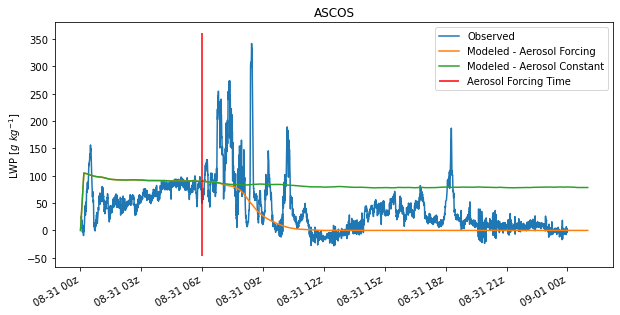
\includegraphics[width=0.45\linewidth]{images/ascos_lwp.png}
	\end{figure}
\end{block}
\end{column}



\begin{column}{\sepwid}\end{column}

\begin{column}{\onecolwid}
	
\end{column}
\begin{column}{\sepwid}\end{column} % Empty spacer column

\end{columns} % End of all the columns in the poster

\end{frame} % End of the enclosing frame

\end{document}
